\chapter{5ta semana - Programar Jugando / La Mansión Maníaca}
\nota{Introducción}{Ya somos capaces de controlar el flujo de un programa, o al menos estamos empezando a hacerlo, además ya entendemos lo que son las instrucciones, las condiciones, etc}
\nota{Objetivo}{Afianzar lo que hicimos. Hasta ahora vimos un montón de cosas. Si hacemos una lista, aprendimos:
\begin{itemize}
  \item Lo que significa programar y a hacer nuestro primer programa en Ruby
  \item A escribir cosas en la pantalla (con \emph{puts})
  \item A sumar, restar y hacer muchas cuentas con la compu, usando números con decimales y enteros (1+4, 3/2, 5*4, etc)
  \item A guardar datos en variables, sin importar si eran palabras o números (a = 'pepe', b = 15)
  \item A leer datos que ingresan en el teclado (con \emph{gets})
  \item A cambiar el rumbo del programa usando condiciones lógicas (usando \emph{if})
\end{itemize}
}
\nota{Cómo lo vamos a hacer}{Vamos a aprender utilizando un nuevo tipo de sentencias, las de un juego que se llama Maniac Mansion. O sea... ¡¡¡vamos a jugar!!!}

\section{Juguemos un poco}
Hay ciertos juegos que se llaman “aventuras de gráficas”. En este tipo de juegos, lo que hay que hacer es tratar de resolver problemas casi detectivescos. Por ejemplo: se nos presenta una situación ficticia, ¡han secuestrado a tu novia! y nosotros somos responsables de rescatarla. Pero en estos juegos, en vez de poner a prueba nuestra destreza con el Joystick, ponen a prueba nuestra destreza mental. Son juegos para pensar. Una de las aventuras más famosas se llama \emph{Maniac Mansion}, así que ¡vamos a ejercitar un poco nuestras habilidades de detectives!

\begin{center}
  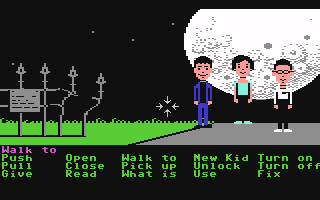
\includegraphics{maniac_mansion_01}
\end{center}

Podemos ver que la imagen que tenemos arriba está dividida en 2 partes: en la parte superior se van dibujando nuestras acciones y en la inferior hay verbos. Para poder hacer algo con nuestros personajes (tenemos 3 para utilizar) tenemos que hacer un click en el verbo (por ejemplo: Abrir) y luego otro click en el objeto (por ejemplo: puerta).\\

El “Maniac Mansion” es un juego clásico que, en la década del 80, fue jugado por miles y miles de chicos y grandes. La clave del éxito era lo difícil de los enigmas, lo novedoso de los gráficos (¡para esa época!) y, por sobre todo, la atrapante historia.

\begin{center}
  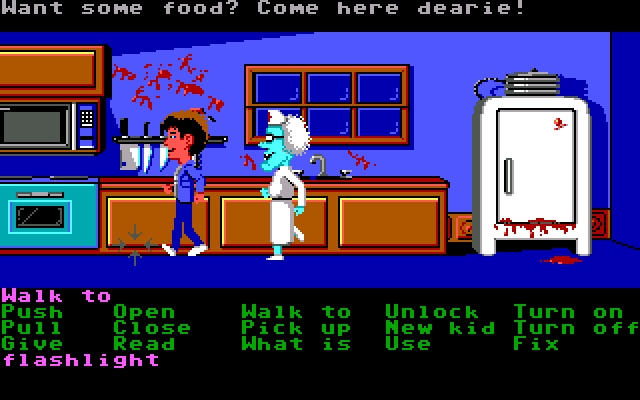
\includegraphics[width=\textwidth]{maniac_mansion_02}
\end{center}

¿Por qué hacemos esto? Hacemos esto porque para resolver este tipo de rompecabezas hay que pensar de la manera que piensan los programadores. Es una manera de aprender: jugando.

\section{Bueno: basta de jugar}
Ahora nos vamos a tomar un tiempo para poder pensar como programaríamos un juego parecido al Maniac Mansion.  ¡Con lo que ya sabemos podemos hacer este juego!\\

Nuestro juego va a ser un poco diferente. Primero vamos a omitir la parte de los gráficos y concentrarnos en los enigmas. Según pudimos ver en el juego, nosotros vamos ingresando nuestras acciones y la computadora nos responde si lo que queremos hacer se puede hacer o no y por qué.\\

Por ejemplo: 
\begin{lstlisting}
puts 'Que queres hacer'
comando = gets.chompputs comando
if (comando == 'ir a escuela') then
  puts('no podes ir a la escuela porque es sabado')
end
\end{lstlisting}

De esta manera validaríamos una acción determinada. Este resultado cambiaría si, por ejemplo, el día fuese distinto. Entonces una mejor manera de escribir esto es la siguiente:

\begin{lstlisting}
dia = 'viernes'
puts 'Que queres hacer'
comando = gets.chomp
puts comando
if (comando == 'ir a escuela' && dia == 'sabado') then
  puts('no podes ir a la escuela porque es sabado')
end
\end{lstlisting}

Así estamos guardando una variable donde ponemos el día en el que estamos y podríamos modificarla si, por ejemplo, nos fuéramos a dormir.